% Options for packages loaded elsewhere
\PassOptionsToPackage{unicode}{hyperref}
\PassOptionsToPackage{hyphens}{url}
%
\documentclass[
]{article}
\usepackage{amsmath,amssymb}
\usepackage{iftex}
\ifPDFTeX
  \usepackage[T1]{fontenc}
  \usepackage[utf8]{inputenc}
  \usepackage{textcomp} % provide euro and other symbols
\else % if luatex or xetex
  \usepackage{unicode-math} % this also loads fontspec
  \defaultfontfeatures{Scale=MatchLowercase}
  \defaultfontfeatures[\rmfamily]{Ligatures=TeX,Scale=1}
\fi
\usepackage{lmodern}
\ifPDFTeX\else
  % xetex/luatex font selection
\fi
% Use upquote if available, for straight quotes in verbatim environments
\IfFileExists{upquote.sty}{\usepackage{upquote}}{}
\IfFileExists{microtype.sty}{% use microtype if available
  \usepackage[]{microtype}
  \UseMicrotypeSet[protrusion]{basicmath} % disable protrusion for tt fonts
}{}
\makeatletter
\@ifundefined{KOMAClassName}{% if non-KOMA class
  \IfFileExists{parskip.sty}{%
    \usepackage{parskip}
  }{% else
    \setlength{\parindent}{0pt}
    \setlength{\parskip}{6pt plus 2pt minus 1pt}}
}{% if KOMA class
  \KOMAoptions{parskip=half}}
\makeatother
\usepackage{xcolor}
\usepackage[left=30mm,right=30mm]{geometry}
\usepackage{graphicx}
\usepackage{float}
\setlength{\footskip}{50pt}
\makeatletter
\def\maxwidth{\ifdim\Gin@nat@width>\linewidth\linewidth\else\Gin@nat@width\fi}
\def\maxheight{\ifdim\Gin@nat@height>\textheight\textheight\else\Gin@nat@height\fi}
\makeatother
% Scale images if necessary, so that they will not overflow the page
% margins by default, and it is still possible to overwrite the defaults
% using explicit options in \includegraphics[width, height, ...]{}
\setkeys{Gin}{width=\maxwidth,height=\maxheight,keepaspectratio}
% Set default figure placement to htbp
\makeatletter
\def\fps@figure{htbp}
\makeatother
\setlength{\emergencystretch}{3em} % prevent overfull lines
\providecommand{\tightlist}{%
  \setlength{\itemsep}{0pt}\setlength{\parskip}{0pt}}
\setcounter{secnumdepth}{-\maxdimen} % remove section numbering
\ifLuaTeX
  \usepackage{selnolig}  % disable illegal ligatures
\fi
\IfFileExists{bookmark.sty}{\usepackage{bookmark}}{\usepackage{hyperref}}
\IfFileExists{xurl.sty}{\usepackage{xurl}}{} % add URL line breaks if available
\urlstyle{same}
\hypersetup{
  pdftitle={Reflective Report},
  hidelinks,
  pdfcreator={LaTeX via pandoc}}

\title{Applied Mathematics for Games Reflective Report - Jacob Costen
(23025180)}
\author{}
\date{}

\begin{document}
\maketitle

\subsection{Summary and Instructions}\label{summary-and-instructions}

The artefact showcases various areas of development of a physics engine:

\begin{itemize}
\tightlist
\item
  Semi-implicit Euler integration for physics modelling, resulting in
  slightly higher stability than explicit Euler
\item
  Multi-threaded physics processing, where physics is processed on a
  separate background thread to rendering, allowing physics to maintain
  a very consistent fixed time step of 60fps.
\item
  Point mass physics: mass, force accumulation, velocity, acceleration,
  gravity, drag, and friction
\item
  Rigid body physics: collision detection and resolution between
  combinations of spherical and axis-aligned bounding box (AABB)
  colliders, including restitution
\item
  Constrained particle physics using spring forces between particles and
  configurable spring length and modulus of elasticity\\
  In addition, the artefact implements an scene tree, objects, and
  components, all of which can be deserialised from a scene file in the
  form of JSON (using a custom JSON parser developed for the project).
  The artefact also includes debugging tools: a system for selecting
  objects in the scene, gizmos to show the origins and orientations of
  each object, and a bounding box to highlight selection; also a
  detailed debug window using my own text user interface library STUI
  (which is header only, immediate mode, and very lightweight, making it
  perfect for this application) to display a terminal-based overview of
  the frame timing, details of the currently selected objects, and
  physics events like collisions.
\end{itemize}

To operate the framework, launch the project and move the debug window
out of the way. Focus the graphical window, and observe the control
scheme below to navigate:\\
WASD - move around (hold shift to move faster)\\
E/Q - move up/down\\
Arrow keys - look around\\
Left click - select object under mouse\\
J/L - apply force to selected object, on X axis\\
I/K - apply force to selected object, on Y axis\\
U/O - apply force to selected object, on Z axis\\
B - reset selected object velocity\\
N - toggle gravity for selected object\\
M - toggle kinematic (affected by collisions) for selected object\\
You can also view these by focusing the debug window and pressing H. The
debug window can be used to view various statistics about the scene,
including the timing of various rendering operations, the length of the
physics tick, the number of objects, meshes, physics components, etc,
and a log of events, specifically physics collision events.

\subsection{UML}\label{uml}

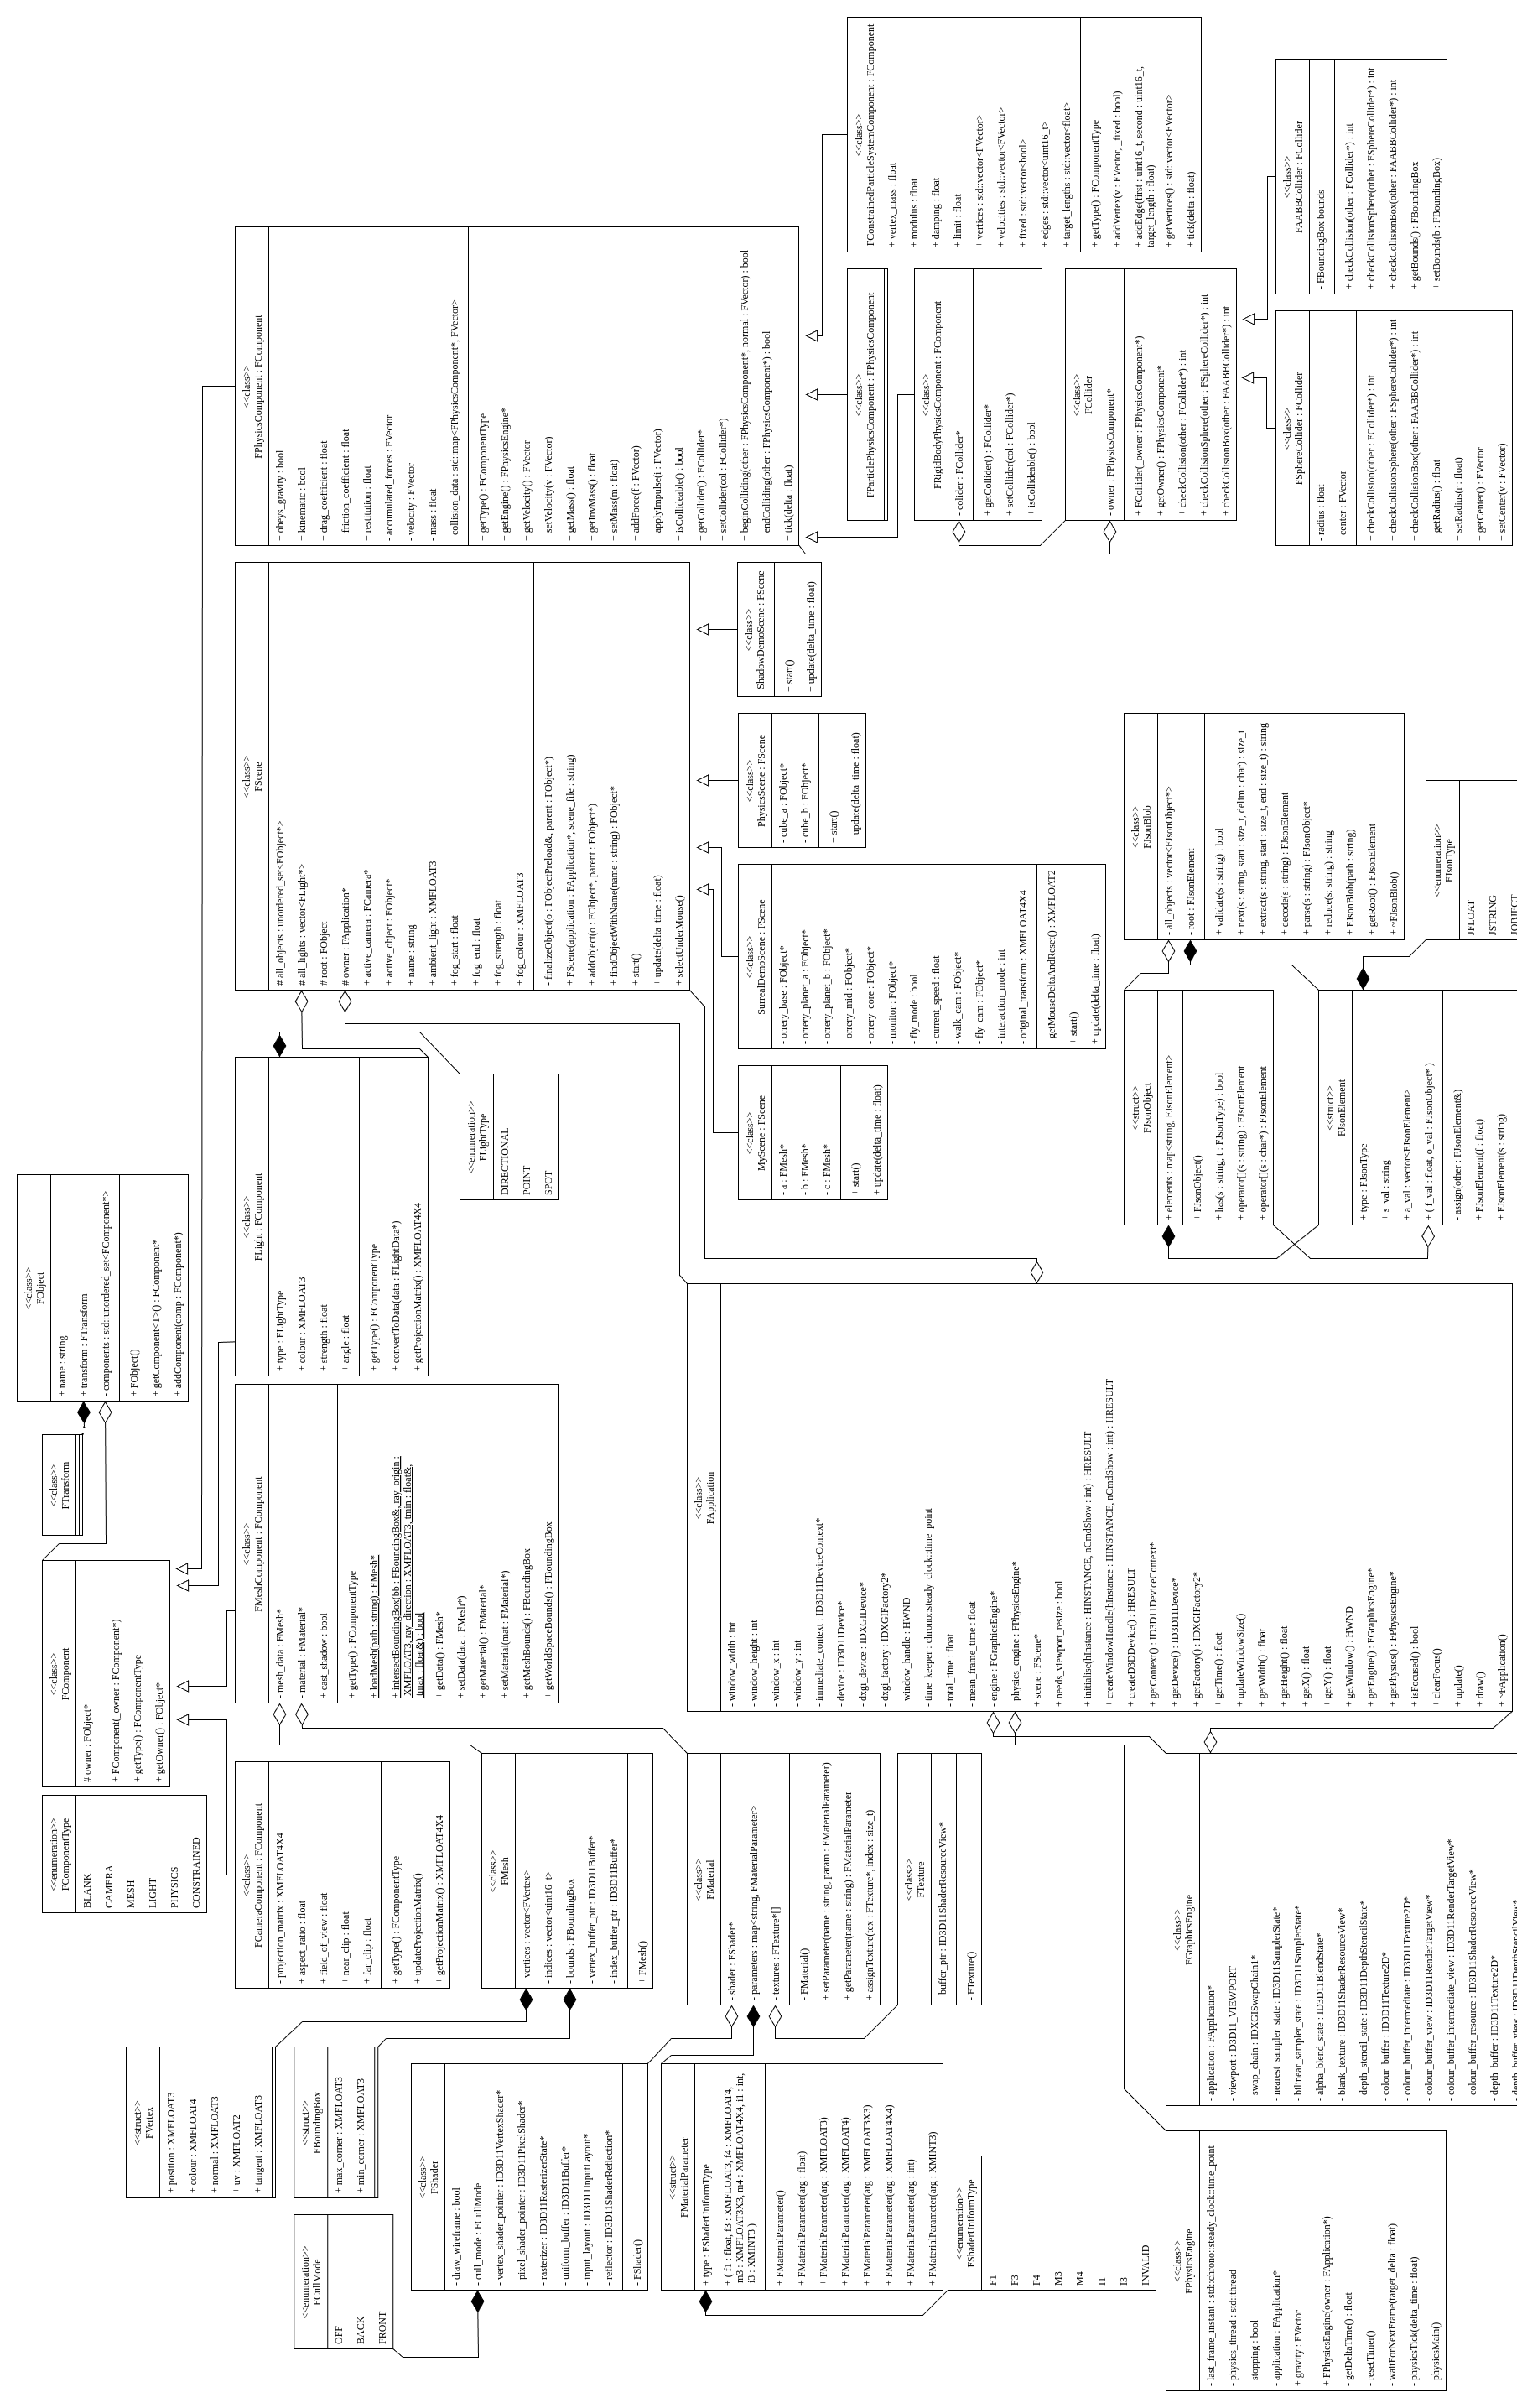
\includegraphics{/mnt/REPOSITORY/Repository-of-Things/Coding/C/framework-renderer/UML_new_a.png}\\
\newline
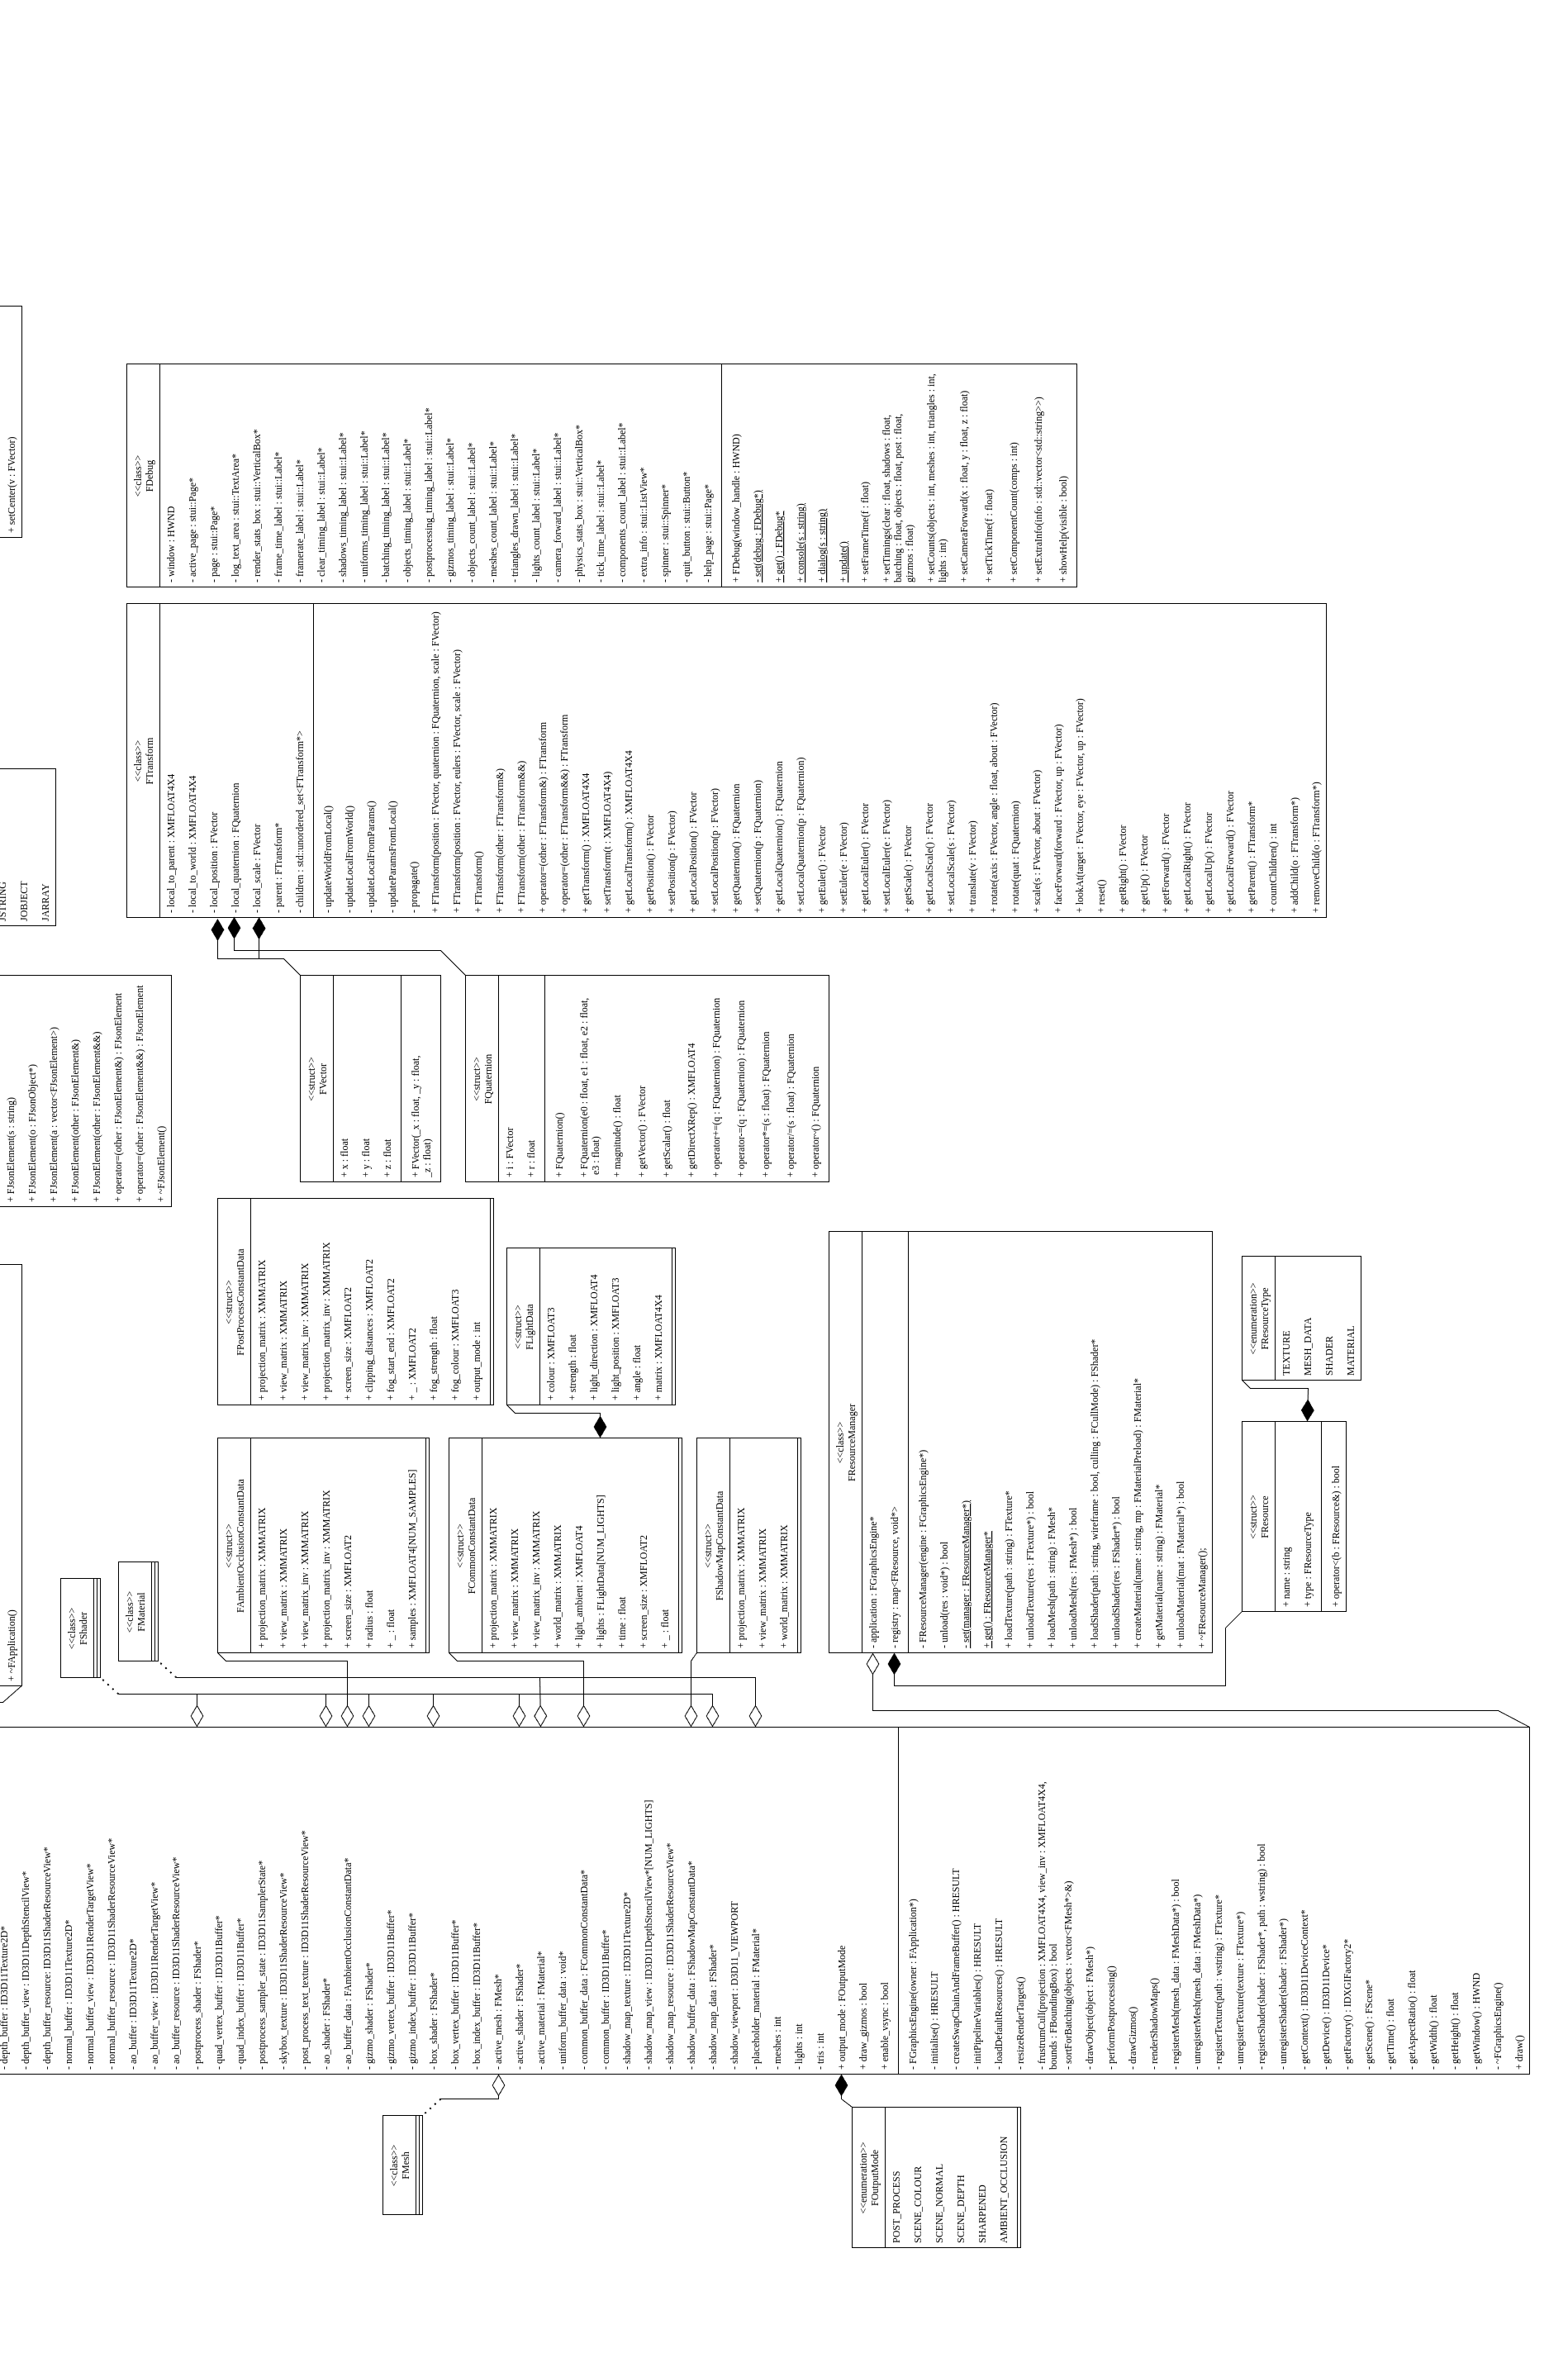
\includegraphics{/mnt/REPOSITORY/Repository-of-Things/Coding/C/framework-renderer/UML_new_b.png}\\

\subsection{Successful Feature}\label{successful-feature}

The framework successfully implements non-oriented rigid bodies. This
supports both collision detection and resolution for collisions between
combinations of AABBs (axis-aligned bounding boxes) and spheres.

The design of this system is such that colliders are separated from the
rigid body itself (i.e. any collider type can be assigned to a rigid
body), and a single collider corresponds to a single physics object, a
model which is common in libraries such as PhysX (Gregory
(2019))\textsuperscript{{[}1{]}}. This fact may be a limitation, since a
common trick in games is to build an object\textquotesingle s collider
out of multiple simple primitives (e.g. two spheres), rather than
building a custom (potentially convex) mesh collider, which would is
almost always more computationally expensive (Ericson
(2005))\textsuperscript{{[}2{]}}\\
Collision detection and resolution were implemented appropriate ways:
sphere-sphere collision is trivial to solve using the relative positions
and combined radii as described by Ericson
(2005)\textsuperscript{{[}2{]}}; sphere-AABB collision is also
relatively simple by computing a nearest-point-on-box. AABB-AABB is more
complex as it involves determining the collision normal based on the
axis with minimum interpenetration (i.e. to estimate which axis it would
be easiest to push the boxes apart along), an approach developed
specifically for the artefact. The use of interpenetration testing in
all three cases means that collision resolution is quite stable.

The rigid body system, implemented in
\texttt{FRigidBodyPhysicsComponent}, inherits behaviour from its parent
\texttt{FPhysicsComponent} class which handles force accumulation,
acceleration, gravity, drag, and friction automatically. This simplifies
the implementation of the rigid body collision system.

As noted above, in addition to course materials, understanding of the
rigid body system was supplemented using Gregory
(2019)\textsuperscript{{[}1{]}} and Ericson
(2005)\textsuperscript{{[}2{]}}, but the Real-Time Rendering website by
Haines (2025)\textsuperscript{{[}4{]}} which provides links to further
resources for implementing intersection detection between various
geometric primitives was also used heavily.

A system for tracking currently colliding objects was also implemented.
Instead of simply returning whether a collision occurred, collider
testing functions return an integer, which represents whether objects
began colliding, continued colliding, or finished colliding. In
addition, each collider contains a \texttt{std::map} of the other
colliders it is currently intersecting, and the collision normal. In a
more advanced form of this feature, the key part of the map would also
store the position at which the collision occurred. This feature was
implemented with reference to Unity\textquotesingle s
\texttt{OnCollisionEnter}, \texttt{OnCollisionExit}, and
\texttt{OnCollisionStay} methods (Unity
(2024))\textsuperscript{{[}3{]}}, which are very useful for implementing
gameplay features on collision (such as sound of visual effects). In the
case of the framework, this also allows the
\texttt{FRigidBodyPhysicsComponent} to compute the frictional forces
affecting it due to ongoing collisions.

Another useful feature of the rigid body system implementation is
support for kinematic bodies. Any physics component can be marked as
kinematic, in which case it ignores forces entirely, as well as
interpenetration response. This makes it easy to
\textquotesingle freeze\textquotesingle{} and object with respect to
physics simulation (although it\textquotesingle s velocity is still
respected), while maintaining the ability for that object to interact
with other objects. This ability is included in reference to similar
options for rigid bodies in Unreal Engine (Epic Games
(2024))\textsuperscript{{[}5{]}} and Unity. In the framework, this
feature is used to create an immovable floor object.

The key feature which is missing from the rigid body system is support
for rotations and oriented bounding boxes (OBBs) in collisions.
Implementation of these would require handling of angular velocity,
optimally using quaternions to express rotations (which eliminates the
problem of Gimbal lock, and eliminates confusion of axis ordering) as
described by Goldman (2011)\textsuperscript{{[}6{]}}, and development of
a new set of collision detection/resolution tests between OBBs and
sphere colliders using the separating axis theorem as described by
Ericson (2005)\textsuperscript{{[}2{]}}.

\subsection{Feature Requiring
Improvement}\label{feature-requiring-improvement}

The framework includes a component for simulating constrained spring
physics, but which was not implemented particularly effectively. The
spring model allows the user to alter the modulus of elasticity, the
damping coefficient, and the minimum and maximum length factor of the
model, as well as being able to define the vertices (point masses) and
edges (spring constraints) between them. In theory this provides a
simple framework from which to build reasonably complex rope or even
cloth systems.

A demonstration scene with a simple double-pendulum-like setup was
created to test the feature, which is essentially a simple rope. Small
sections of cloth-like configurations (with structure and shear springs
as described by Bourg and Bywalec (2013)\textsuperscript{{[}8{]}}) were
also tested, but were far too unstable to meaningfully demonstrate the
feature.

The key problem with the spring physics system is that it suffers very
heavily from computational inaccuracy and poor stability in integration.
Points affected by multiple forces tend to jitter violently unless heavy
damping is applied, and springs may oscillate where otherwise they would
come to rest in equilibrium. This is fundamentally due to the
integration method used being a semi-implicit Euler method, which while
being simple to implement and efficient in this case, leads to an
unstable simulation, as backed up by the findings of Galachenko, et al.
(2024)\textsuperscript{{[}7{]}} who found similar results with another
numerical integration problem.

The problem arises from the fact that a spring may be under a certain
amount of tension, and thus produce a certain force to resolve that.
However, without sufficiently small timesteps, the spring will overshoot
its contraction due to the applied force and by the time the next
timestep occurs, it will be far enough in compression that it must be
stretched again with a similar force. This insufficient granularity of
simulation leads to the jittering and instability observed both in the
framework and in other studies covering numerical integration of systems
of related equations.

In an attempt to improve stability, and as an additional feature, the
ability to clamp the length of the spring was added. This allows the
user to specify a fraction of the rest length of the spring at which the
spring cannot become shorter, and this restriction was implemented by
altering the force applied to points during solving to prevent (or
attempt to prevent) the connecting edge from becoming shorter than {} or
longer than {}. However, testing showed that if this clamping mechanism
was activated too frequently (particularly on successive frames), or if
the upper and lower limits were too close together, the simulation would
actually become much less stable and jittering of points would be much
worse.

One element of this feature which was implemented successfully was
pinning: this allows select vertices to be fixed in place, and spring
forces will only be applied to the other end of each spring, which is a
useful feature present in many applications supporting cloth
simulations, for example Blender (2025)\textsuperscript{{[}9{]}} which
actually allows users to specify a degree to which each vertex is
pinned, giving a greater degree of control than is present in the
framework.

The solution to improve the quality and stability of the simulation
would be to use a more effective integration method. The best choice
would be a Runge-Kutta technique, specifically RK4 which is commonly
used in videogame physics engines due to its high stability and
consistent convergence to a solution, balanced with not being too
computationally expensive as illustrated by Hauth
(2003)\textsuperscript{{[}10{]}}. Runge-Kutta represents a Taylor series
expansion of the expression defining acceleration at different points
along the timeline between the beginning and end of the timestep, which
are then used to calculate an estimated overall gradient between the
start and end, hence giving a more accurate result. Runge-Kutta is also
open to further improvement in terms of speed and efficiency, as shown
by Wang, Hu, and Zhuang (2009)\textsuperscript{{[}11{]}} who produced a
6-iteration (rather than 4) Runge-Kutta method which supports dynamic
timesteps (in fact, the wider timesteps possible with Runge-Kutta are
what allows it to be more less computationally expensive) and solves a
test scenario in barely half the time of RK4. The one downside to RK4 is
that it tends to lose energy compared to semi-implicit integration
(Fielder (2004))\textsuperscript{{[}12{]}}, which could become a problem
in this spring physics application, where an additional damping force is
also applied.

It would almost certainly be best to implement this new integration
method using DirectX\textquotesingle s math functions, rather than the
framework\textquotesingle s custom \texttt{FVector} implementation. This
will allow the more advanced integration to take advantage of
DirectX\textquotesingle s use of SIMD (single instruction multiple data)
instructions.

\subsection{Bibliography}\label{bibliography}

{[}1{]}: Gregory, J. (2019) \emph{Game Engine Architecture}. 3rd edn.
Boca Raton, FL: CRC Press, Taylor \& Francis Group.\\
{[}2{]}: Ericson, C. (2005) \emph{Real-time collision detection}.
Amsterdam: Elsevier.\\
{[}3{]}: Technologies, Unity (2024)
\textquotesingle Collider\textquotesingle, \emph{Unity}. Available at:
\url{https://docs.unity3d.com/6000.0/Documentation/ScriptReference/Collider.html}
(Accessed: 12 February 2025).\\
{[}4{]}: Haines, E. (2025) \textquotesingle Ray Tracing
Resources\textquotesingle, \emph{Real-Time Rendering}. Available at:
\url{https://www.realtimerendering.com/intersections.html} (Accessed: 12
February 2025).\\
{[}5{]}: Games, Epic (2024) \textquotesingle Physics bodies
reference\textquotesingle, \emph{Unreal Engine Documentation}. Available
at:
\url{https://dev.epicgames.com/documentation/en-us/unreal-engine/physics-bodies-reference-for-unreal-engine}
(Accessed: 12 February 2025).\\
{[}6{]}: Goldman, R. (2011) `Understanding quaternions', \emph{Graphical
Models}, 73(2), pp. 21--49. doi:10.1016/j.gmod.2010.10.004.\\
{[}7{]}: Galchenko, M. \emph{et al.} (2024) `Semi-implicit numerical
integration of Boundary Value Problems', \emph{Mathematics}, 12(23), p.
3849. doi:10.3390/math12233849.\\
{[}8{]}: Bourg, D.M. and Bywalec, B. (2013) \emph{Physics for game
developers}. 2nd edn. Sebastopol, Calif: O'Reilly Media.\\
{[}9{]}: Blender (2025) \textquotesingle Shape\textquotesingle,
\emph{Blender 4.3 Manual}. Available at:
\url{https://docs.blender.org/manual/en/latest/physics/cloth/settings/shape.html}
(Accessed: 12 February 2025).\\
{[}10{]}: Hauth, M., (2003) \textquotesingle Numerical techniques for
cloth simulation\textquotesingle~\emph{SIGGRAPH
\textquotesingle Clothing Simulation and Animation\textquotesingle{}}\\
{[}11{]}: Wang, J., Hu, X. and Zhuang, Y. (2009) `The dynamic cloth
simulation performance analysis based on the improved spring-mass
model', \emph{2009 International Conference on Wireless Networks and
Information Systems}, pp. 282--285. doi:10.1109/wnis.2009.41.\\
{[}12{]}: Fielder, G. (2004) \textquotesingle Integration
basics\textquotesingle, \emph{Gaffer On Games}. Available at:
\url{https://gafferongames.com/post/integration_basics/} (Accessed: 12
February 2025).

\end{document}
